% -*- mode: fundamental -*-

% ****************************************************************

\chapter{RISC-V: the Fife pipelined CPU: BSV code}

\markboth{Ch \arabic{chapter}: Fife BSV code (DRAFT)}{\copyrightnotice}

\setcounter{page}{1}
% \renewcommand{\thepage}{\arabic{page}}
\renewcommand{\thepage}{\arabic{chapter}-\arabic{page}}

\label{ch_Fife_Code}

% ****************************************************************

\section{Introduction}

In this chapter we look at the BSV code to implement the principles
discussed in the previous chapter.  We repeat
Figure~\ref{Fig_Instr_Exec_w_FIFOs} for reference.

\begin{figure}[htbp]
  \centerline{\includegraphics[width=6in,angle=0]{Figures/Fig_Instr_Exec_w_FIFOs}}
  \caption{\label{Fig_Instr_Exec_w_FIFOs_2}Pipelined interpretation of RISC-V instructions (Fig.~\ref{Fig_Instr_Exec} with some annotations)}
\end{figure}

% ****************************************************************

\section{Fife: CSRs}

To be written ...

\begin{tightlist}
\item CSRRxx are read-modify-write operations
\item CSRRxx access may not be memory-like (side-effecting reads, read
      may not return last written value,
\item ... (a bit like MMIO issues)
\end{tightlist}
Hard to pipeline, so execute in Retire stage, as FSM.

CSRRxx instructions should be rare, so FSM exec does not affect overall performance.

% ****************************************************************

\section{Fife: Interrupts}

To be written ...

Check for interrupts in Retire stage, fix up CSRs and and redirect.

Retire stage already has infra for CSR update and redirection, so this
is a small incremental change.

% ****************************************************************
